% ============================================================
% CAPÍTULO 4
% ============================================================
\capitulo{Desarrollo Experimental: Materiales, Métodos y Algoritmos}

Este capítulo describe con el detalle necesario para reproducirlo todo lo que se hizo desde el video crudo hasta la aplicación de inferencia: los materiales, el conjunto de datos, el preprocesamiento, los cuatro candidatos que se compararon, el protocolo con el que se los evaluó y la historia del desarrollo que condujo a ese protocolo. Los resultados se presentan en el Capítulo~5; los caminos que se exploraron y se descartaron, en el Anexo~C; y la devolución del docente y lo que se hizo con ella, en el Anexo~D.

\section{Materiales}
El sistema se implementó en Python 3.10 con PyTorch \parencite{paszke2019}, scikit-learn \parencite{pedregosa2011}, OpenCV \parencite{bradski2000} y DeepLabCut \parencite{mathis2018}, que se utilizó con el modelo preentrenado SuperAnimal-Quadruped \parencite{ye2024}. La interfaz se construyó con Streamlit. La estimación de pose y la extracción de características visuales se ejecutaron en una computadora local con una GPU NVIDIA RTX 3070 de 8~GB; el modelado posterior no requiere GPU, salvo el entrenamiento del modelo de atención sobre instancias (MIL, por \textit{multiple instance learning}), que es pequeño y también corre en ella. El entorno se aisló en un entorno virtual con las versiones fijadas en el repositorio.

El código, las pruebas automatizadas (\texttt{tests/}), los protocolos y la documentación se versionaron en un repositorio Git (\url{https://github.com/sergioyanez/Tesina-UGR}). Los videos crudos y los artefactos pesados (fotogramas, coordenadas de pose, características, modelos entrenados) se mantienen fuera del repositorio, en rutas que se declaran por variables de entorno; cada resultado de la comparación lleva la huella del conjunto de datos, de las particiones y de la reserva con que se generó.

\section{Conjunto de Datos}
No existía un conjunto público con estas tres clases, por lo que se construyó uno propio a partir de videos filmados con teléfono celular en la región de Tandil (provincia de Buenos Aires). Los videos se organizaron en carpetas por clase y el identificador del caballo se tomó del prefijo numérico del nombre de archivo; ese identificador es la unidad de agrupamiento que permite particionar sin fuga de información \parencite{kapoor2023}.

\subsection{Videos, Sesiones de Filmación y Clips}
Se catalogaron \VideosTotal{} videos originales. Para poder evaluar la generalización a situaciones de filmación nuevas se reconstruyó, a partir de la fecha y la hora de cada video (tomadas del nombre del archivo o, si éste no la traía, de los metadatos), la sesión de filmación a la que pertenece: un conjunto de videos obtenidos en el mismo lugar y momento. Los videos sin fecha deducible se asignaron a su sesión manualmente. El resultado son \SesionesTotal{} sesiones, todas registradas con Tandil como localidad de referencia, resumidas en la Tabla~\ref{tab:c4-sesiones}.

\begin{table}[H]
\caption{Sesiones de filmación confirmadas}\label{tab:c4-sesiones}
{\singlespacing\small
\begin{tabular}{@{}llrrrrrl@{}}
\toprule
Sesión & Fecha & Videos & Caballos & \clase{Disg.} & \clase{Int.} & \clase{Ser.} & Resolución \\
\midrule
S001 & 04--05/04/2015 & 13 & 11 & 1 & 12 & 0 & 640$\times$480 \\
S003 & 03/03/2023 & 1 & 1 & 0 & 1 & 0 & 720$\times$1280 \\
S004 & 14/03/2023 & 1 & 1 & 0 & 0 & 1 & 1080$\times$1920 \\
S005 & 14/04/2023 & 1 & 1 & 0 & 1 & 0 & 1080$\times$1920 \\
S006 & 28/04/2023 & 15 & 8 & 7 & 6 & 2 & 1080$\times$1920 \\
S008 & 30/06/2023 & 4 & 3 & 2 & 1 & 1 & 1080$\times$1920 \\
S009 & 03/07/2023 & 1 & 1 & 0 & 1 & 0 & 1080$\times$1920 \\
S010 & 24/11/2023 & 1 & 1 & 0 & 0 & 1 & 1080$\times$1920 \\
S011 & 04/10/2025 & 13 & 13 & 2 & 8 & 3 & 1080$\times$1920 \\
S012 & 04/10/2025 & 4 & 4 & 0 & 4 & 0 & 1080$\times$1920 \\
S013 & 12/05/2026 & 2 & 1 & 2 & 0 & 0 & 2560$\times$1440 \\
S014 & 15/05/2026 & 2 & 1 & 2 & 0 & 0 & 2560$\times$1440 \\
S015 & 01/07/2026 & 5 & 2 & 3 & 2 & 0 & 1080$\times$1920 \\
S016 & 02/07/2026 & 14 & 7 & 6 & 5 & 3 & 1080$\times$1920 \\
S017 & 02/07/2026 & 50 & 13 & 17 & 13 & 20 & 1080$\times$1920 \\
S018 & 07/07/2026 & 17 & 8 & 0 & 1 & 16 & 1080$\times$1920 \\
S019 & 11/08/2026 & 17 & 9 & 2 & 3 & 12 & 1080$\times$1920 \\
S020 & 18/08/2026 & 77 & 43 & 30 & 13 & 34 & 1080$\times$1920 \\
S021 & 26/08/2026 & 4 & 2 & 4 & 0 & 0 & 2560$\times$1440 \\
S022 & 27/08/2026 & 7 & 5 & 7 & 0 & 0 & 2560$\times$1440 \\
S023 & 02/09/2026 & 7 & 4 & 7 & 0 & 0 & 1080$\times$1920 \\
S024 & 03/09/2026 & 18 & 9 & 18 & 0 & 0 & 1080$\times$1920 \\
\bottomrule
\end{tabular}}
\notatabla{Cantidad de videos originales (\VideosTotal{} en total) por sesión, caballos distintos filmados en ella y videos por clase (\clase{Disg.} = \clase{Disgustado}, \clase{Int.} = \clase{Interesado}, \clase{Ser.} = \clase{Sereno}). Los identificadores conservan la numeración de la propuesta inicial de agrupamiento; los que faltan (S002, S007) se fusionaron con la sesión contigua al confirmarlas. La sesión S020 concentra 77 de los \VideosTotal{} videos y las sesiones S023 y S024 sólo contienen \clase{Disgustado}.}
\end{table}

Cada video se segmenta en ventanas de alrededor de 6~s sin solapamiento, que absorben un resto final de hasta 7~s; la duración mínima para conservar un video corto se fijó en 1~s para no descartar de manera preferencial la clase \clase{Disgustado}, cuyas tomas son breves. De este proceso resultaron 393 clips candidatos, de los cuales \ClipsTotal{} ofrecen una secuencia utilizable (ver el apartado de selección de fotogramas). Esos \ClipsTotal{} clips íntegros, de \CaballosTotal{} caballos, son el conjunto con el que se trabajó (Tablas~\ref{tab:c4-tamano} y~\ref{tab:c4-clases}).

\begin{table}[H]
\caption{Tamaño del conjunto de datos}\label{tab:c4-tamano}
{\singlespacing
\begin{tabular}{@{}lr@{}}
\toprule
Elemento & Cantidad \\
\midrule
Videos originales catalogados & \VideosTotal{} \\
Sesiones de filmación & \SesionesTotal{} \\
Clips candidatos & 393 \\
Clips utilizados & \ClipsTotal{} \\
Caballos distintos & \CaballosTotal{} \\
\bottomrule
\end{tabular}}
\notatabla{Un clip candidato se descarta cuando no contiene una ventana con suficientes fotogramas medidos. Se utiliza el 91,3~\% de los candidatos.}
\end{table}

\begin{table}[H]
\caption{Distribución por clase de los clips utilizados}\label{tab:c4-clases}
{\singlespacing
\begin{tabular}{@{}lrrrr@{}}
\toprule
Clase & Desarrollo & Reserva & Total & Caballos \\
\midrule
\clase{Disgustado} & \ClipsDevDisg{} & \ClipsReservaDisg{} & 103 & 57 \\
\clase{Interesado} & \ClipsDevInt{} & \ClipsReservaInt{} & 118 & 60 \\
\clase{Sereno} & \ClipsDevSer{} & \ClipsReservaSer{} & 138 & 52 \\
\midrule
Total & \ClipsDesarrollo{} & \ClipsReserva{} & \ClipsTotal{} & \CaballosTotal{} \\
\bottomrule
\end{tabular}}
\notatabla{Las columnas «Desarrollo» y «Reserva» corresponden a la partición descrita en el protocolo de evaluación (\CaballosDesarrollo{} y \CaballosReserva{} caballos, respectivamente). La suma de caballos por clase supera \CaballosTotal{} porque 29 animales aparecen en más de una clase (22 en dos y 7 en las tres): la etiqueta describe un momento, no al individuo.}
\end{table}

\subsection{Etiquetado}
Cada clip fue etiquetado como \clase{Sereno}, \clase{Interesado} o \clase{Disgustado} por una veterinaria con certificación como codificadora del sistema de codificación de acciones faciales equinas \parencite[EquiFACS;][]{wathan2015}, siguiendo un protocolo escrito (\texttt{docs/protocolo\_de\_etiquetado.md}) que traduce los criterios de la Tabla~\ref{tab:c2-criterio} en reglas observables sobre orejas, ojos, boca y movimiento de cabeza. Se trata de un único observador y no se midió el acuerdo interobservador sobre el conjunto; sólo se realizó un piloto sobre imágenes, con un valor de kappa de Fleiss \parencite{fleiss1971} de 0,99 que no puede extrapolarse a los videos. Los estados emocionales no se infieren: se predicen categorías definidas por el protocolo, con las limitaciones que se discuten en el Capítulo~5.

\subsection{Problemas Detectados en los Datos}
Durante la construcción del conjunto se detectaron y corrigieron: un video duplicado en dos clases, videos con la orientación guardada como metadato, una copia local incompleta de la fuente de datos, archivos auxiliares de DeepLabCut mezclados con los clips, desenfoque de movimiento y cabezas parcialmente fuera de cuadro. Se adoptó una única fuente de datos declarada, corrección automática de la orientación y controles de duplicados.

Persisten tres problemas que no pudieron corregirse y que condicionan la interpretación de los resultados:

\begin{itemize}
  \item \textbf{Duración distinta por clase.} La mediana de duración de los clips es de 3,2~s en \clase{Disgustado} y de 6,0~s en \clase{Interesado} y \clase{Sereno}; el 33,4~\% de los clips (120 de \ClipsTotal{}) dura menos de 5~s. Es coherente con el contexto de filmación ---las interacciones que originan \clase{Disgustado} son breves y bruscas---, pero es una señal que un modelo podría aprovechar sin mirar la cara.
  \item \textbf{Formato distinto por clase.} Los videos de 640$\times$480 corresponden sólo a \clase{Interesado} (26 clips) y \clase{Disgustado} (2); los de 2560$\times$1440, sólo a \clase{Disgustado} (8). \clase{Sereno} es 100~\% 1080$\times$1920. Un modelo podría, en principio, reconocer la clase por el formato de filmación, un atajo del tipo descrito por \textcite{geirhos2020}.
  \item \textbf{Identidades repetidas.} Los caballos 123 y 169 resultaron ser el mismo animal con dos identificadores (dos videos de \clase{Interesado} filmados con 34~s de diferencia el 04/10/2025, cuya identidad se confirmó comparando fotogramas). Las particiones ya estaban fijadas cuando se detectó; se midió el efecto y no modifica ningún resultado (Capítulo~5).
\end{itemize}

Para controlar los dos primeros se definió, antes de comparar modelos, un \textit{subconjunto limpio}: los clips de \CriterioLimpio, que no delatan la clase por el formato ni por la duración. Contiene \ClipsLimpioDesarrollo{} clips de \CaballosLimpioDesarrollo{} caballos en el desarrollo y \ClipsLimpioReserva{} clips en la reserva, y todos los resultados se informan también sobre él.

\section{Preprocesamiento}
La Figura~\ref{fig:c4-pipeline} resume el recorrido que sigue cada clip desde el video hasta la clase predicha. Las etapas se describen a continuación.

\begin{figure}[H]
\caption{Esquema del sistema de clasificación de la expresión facial}\label{fig:c4-pipeline}
\centering
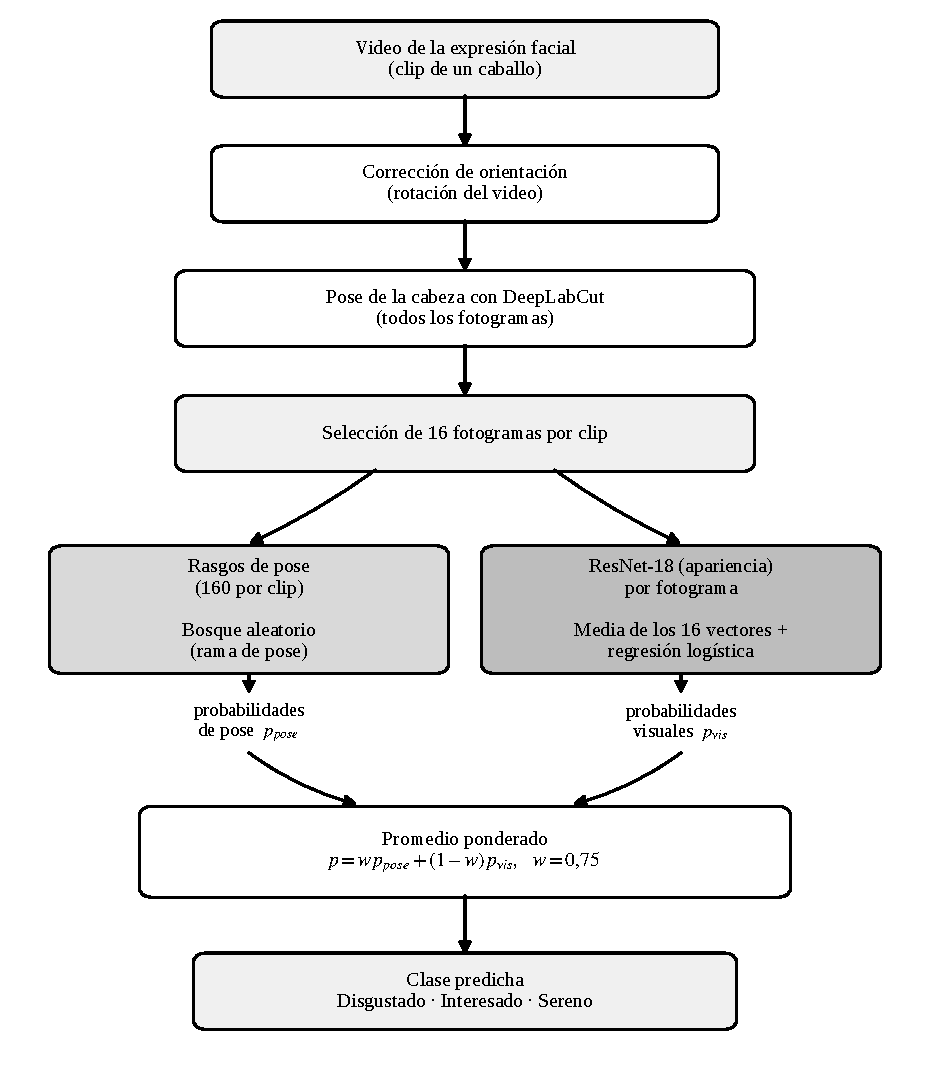
\includegraphics[width=\textwidth]{figuras/pipeline.pdf}
\notatabla{Los \PoseRasgos{} rasgos de pose se calculan con las coordenadas de DeepLabCut; la rama visual usa ResNet-18 sobre \Fotogramas{} fotogramas por clip. El peso de la pose, $w$ = \PesoPose{}, se elige por validación interna (\PesoPose{} en \PesoFoldsA{} de \PesoFoldsTotal{} pliegues).}
\end{figure}

\subsection{Orientación del Video}
Muchos teléfonos guardan el video sin rotar y registran la orientación como metadato. De los \VideosTotal{} videos, 69 tienen una rotación de 90 grados. Si el decodificador la ignora, el detector recibe la cara acostada y falla; en una medición temprana, los videos rotados perdían más de la mitad de sus fotogramas medidos. Se resolvió activando la corrección automática de OpenCV (\texttt{CAP\_PROP\_ORIENTATION\_AUTO}) en todas las lecturas, tanto en el entrenamiento como en la aplicación.

\subsection{Estimación de Pose sobre Todos los Fotogramas}
DeepLabCut se ejecutó con el modelo SuperAnimal-Quadruped sin ajuste, sobre todos los fotogramas de los 393 clips candidatos (alrededor de 73\,000). Una versión temprana ubicaba la cabeza con un detector de objetos YOLO \parencite{redmon2016,jocher2024}; en la versión vigente el encuadre se calcula con el ojo y el hocico estimados por la pose y el detector no participa. No se usó el subconjunto específico para caballos (Horse-30) ni se midió la calidad de los puntos frente a una anotación humana del conjunto; ambas son limitaciones declaradas. Es la etapa más costosa, pero se ejecuta una sola vez y su resultado se almacena, lo que permite cambiar el criterio de selección de fotogramas sin repetir el cálculo.

\subsection{Selección de los 16 Fotogramas}
Una primera versión fijaba 16 posiciones equiespaciadas antes de saber qué fotogramas tenían mediciones válidas; un fotograma fallido se recuperaba por interpolación o anotación manual, y con ese enfoque sólo 153 de los 393 clips resultaban utilizables. La versión vigente invierte el orden: primero mide y después elige. El algoritmo (a) busca la ventana temporal más larga, de hasta 7~s, que contenga al menos \Fotogramas{} fotogramas válidos y ningún hueco sin medición mayor a 0,5~s; (b) distribuye \Fotogramas{} posiciones equiespaciadas en esa ventana, y (c) ancla cada posición al fotograma válido de mayor confianza dentro de una tolerancia de 0,10~s. No se interpolan puntos ni se anotan fotogramas a mano: si un clip no ofrece una ventana suficiente, se descarta. Este cambio elevó los clips utilizables de 153 a \ClipsTotal{} sin filmar videos nuevos. Un fotograma es válido cuando la confianza de ojo y hocico es de al menos 0,50, el mismo umbral que se usa para construir las máscaras de validez de los puntos faciales (un punto con confianza menor se considera ausente).

\subsection{Representación Visual}
Cada fotograma seleccionado se alinea a partir de la posición del ojo y del hocico, se recorta con un encuadre de $224 \times 343$ píxeles que incluye las orejas, se guarda en JPEG con calidad 95 y se procesa con una ResNet-18 \parencite{he2016} preentrenada en ImageNet \parencite{deng2009} y congelada, que produce 512 características por fotograma. Cada clip queda representado por una matriz de \Fotogramas{}$\times$512. La aplicación de inferencia reproduce exactamente este recorrido, incluida la compresión, para que el modelo reciba en producción la misma distribución de imágenes que en el entrenamiento. Se probó entrenar parcialmente la ResNet-18 y no se obtuvo mejora distinguible (Anexo~C), por lo que el extractor permanece congelado.

\subsection{Representación de Pose}
La rama de pose parte de las coordenadas de ojos, hocico, orejas, mandíbula y comisuras de los mismos \Fotogramas{} fotogramas y produce dos representaciones.

\textbf{Rasgos tipo SimBA (\PoseRasgos{} por clip).} Siguiendo el estilo de rasgos que calcula SimBA \parencite{goodwin2024} a partir de una tabla de puntos ---distancias, ángulos, razones, velocidades y aceleraciones, con estadísticos agregados---, se programaron rasgos propios, porque los extractores de SimBA no son aplicables a este esquema de puntos; por eso el informe los llama «rasgos tipo SimBA» y no SimBA. Se agrupan en 130 rasgos estáticos (26 series por fotograma resumidas con media, desvío, mínimo, máximo y rango), 21 dinámicos (7 series de velocidad y aceleración resumidas con media, desvío y máximo) y 9 de disponibilidad (qué fracción de los fotogramas tiene medido cada punto). Todas las longitudes se dividen por la escala del clip, definida como la mediana de la distancia ojo--hocico entre sus fotogramas válidos; así no hay estadística global y no se filtra información entre pliegues. Un punto con confianza menor de 0,50 se trata como ausente: alrededor del 14~\% de los valores falta y se imputa con la mediana del entrenamiento dentro de cada pliegue.

\textbf{Geometría v2 (17 columnas por fotograma).} Es la descripción que usa el MIL. Todo se expresa en el marco de la cabeza (eje $x$ del ojo al hocico, escala igual a esa distancia en el fotograma): largo y ángulo de cada oreja (4 columnas), vector hocico--mandíbula (2), ancho de boca (1), distancia interocular (1), escorzo (1), seno y coseno de la inclinación de la cabeza (2) y seis máscaras de validez con umbral de confianza de 0,50. La versión anterior (v1, 9 columnas) llevaba esencialmente un solo grado de libertad ---la inclinación de la cabeza--- y máscaras que valían 1 en todos los fotogramas por usar un umbral de confianza nulo; la v2 corrige ambas cosas. Es una descripción 2D de una cámara, por lo que depende del punto de vista, y no fue validada con un especialista.

\section{Los Cuatro Candidatos}
Se compararon cuatro modelos de complejidad creciente, todos con la misma entrada de datos, las mismas particiones y el mismo evaluador. La Tabla~\ref{tab:c4-candidatos} los resume, con su orden de simplicidad (1 = más simple), que es el que utiliza la regla de desempate del criterio de elección. Los hiperparámetros se fijaron antes de medir y no se ajustaron con ningún conjunto de prueba; los que se eligen dentro de un candidato se eligen con una validación interna.

\begin{table}[H]
\caption{Candidatos de la comparación}\label{tab:c4-candidatos}
{\singlespacing\small
\begin{tabularx}{\textwidth}{@{}clXlc@{}}
\toprule
N.º & Candidato & Descripción & Entrada & Simplicidad \\
\midrule
1 & Línea de base & Regresión logística sobre la media de los \Fotogramas{} vectores visuales & Visual & 1 \\
2 & Bosque aleatorio de pose & Bosque aleatorio (\textit{random forest}) sobre los \PoseRasgos{} rasgos tipo SimBA & Pose & 2 \\
3 & Fusión pose + visual & Promedio ponderado de las probabilidades de los dos anteriores & Pose y visual & 3 \\
4 & MIL multimodal corregido & Red con atención sobre los \Fotogramas{} fotogramas & Visual y pose & 4 \\
\bottomrule
\end{tabularx}}
\notatabla{La simplicidad es una escala ordinal fijada en el protocolo antes de comparar: cuenta qué tan simple es el modelo en cantidad de componentes y de parámetros y en la facilidad de explicar su salida.}
\end{table}

\subsection{Candidato 1. Línea de Base sobre la Media Visual}
Se promedian los \Fotogramas{} vectores de 512 características de cada clip, se estandarizan (media y desvío calculados sólo con el entrenamiento del pliegue) y se ajusta una regresión logística multinomial con regularización $C = 0{,}1$, pesos de clase balanceados y hasta 5\,000 iteraciones. Es el modelo más simple y ignora tanto el orden como la pose; sirve de referencia para saber qué aporta cada componente adicional.

\subsection{Candidato 2. Bosque Aleatorio de Pose}
Sobre los \PoseRasgos{} rasgos tipo SimBA se ajusta un bosque aleatorio \parencite{breiman2001} de 500 árboles, con \texttt{max\_features} igual a la raíz del número de rasgos, hojas de al menos 2 muestras (\texttt{min\_samples\_leaf} = 2), pesos de clase balanceados y semilla 0, precedido de una imputación por la mediana del entrenamiento. Estos hiperparámetros se habían fijado en la auditoría, antes de la comparación, y no se eligieron mirando datos de prueba.

\subsection{Candidato 3. Fusión Tardía de Pose y Apariencia}
La fusión combina las probabilidades de los dos modelos anteriores \parencite[fusión de clasificadores;][]{kittler1998}, según la ecuación~(\ref{eq:c3-fusion}) del Capítulo~3, con la notación siguiente:
\[
p = w\,p_{\mathrm{pose}} + (1-w)\,p_{\mathrm{visual}},
\]
donde $p_{\mathrm{pose}}$ es la salida del bosque aleatorio y $p_{\mathrm{visual}}$ la de la regresión logística. El peso $w$ pertenece al conjunto $\{0;\,0{,}25;\,0{,}5;\,0{,}75;\,1\}$ y se elige dentro de cada ajuste con una validación interna por caballo de 4 pliegues (\texttt{StratifiedGroupKFold}, semilla 0) sobre el entrenamiento, maximizando la \fmacro{} de las probabilidades fuera de muestra; si hay empate se prefiere el peso más cercano a 0,5. Una vez elegido $w$, ambos modelos se reentrenan con todo el entrenamiento. La variante tardía se fijó antes de mirar resultados de prueba y la variante temprana (concatenar rasgos) no se evaluó. En las 20 evaluaciones del desarrollo el peso elegido fue \PesoPose{} en \PesoFoldsA{} de \PesoFoldsTotal{} pliegues y \PesoPoseUno{} en el restante: la fusión está dominada por la pose.

\subsection{Candidato 4. MIL Multimodal Corregido}
Es el modelo con que se trabajó hasta el 07/10, con tres correcciones que surgieron de la auditoría: geometría v2 en lugar de v1, máscaras de validez con umbral 0,50 y validación interna estratificada por caballo y por clase. En el aprendizaje con múltiples instancias \parencite{ilse2018} cada clip es una «bolsa» de \Fotogramas{} fotogramas y el modelo aprende cuánto pesa cada uno. La arquitectura es la siguiente: por cada fotograma, el vector geométrico de 17 columnas pasa por un perceptrón multicapa $17 \rightarrow 64 \rightarrow 128$ con activaciones ReLU y se concatena con las 512 características visuales (640 dimensiones); una red de atención ($640 \rightarrow 128 \rightarrow 1$, con tangente hiperbólica) asigna un puntaje a cada fotograma, que una softmax con máscara convierte en pesos; la suma ponderada forma la representación del clip, que un clasificador $640 \rightarrow 64 \rightarrow 3$ convierte en puntajes por clase. Tiene 132\,867 parámetros entrenables, sin contar la ResNet-18. Como la atención es una suma ponderada, el modelo es invariante al orden de los fotogramas: se verificó numéricamente que barajar o invertir los \Fotogramas{} fotogramas no cambia ninguna de las \ClipsTotal{} predicciones, de modo que agrega información de varias imágenes pero no modela la evolución temporal.

La Tabla~\ref{tab:c4-hiper} reúne los hiperparámetros de entrenamiento.

\begin{table}[H]
\caption{Hiperparámetros del MIL multimodal corregido}\label{tab:c4-hiper}
{\singlespacing
\begin{tabular}{@{}ll@{}}
\toprule
Parámetro & Valor \\
\midrule
Optimizador & Adam, tasa de aprendizaje $10^{-3}$, decaimiento de pesos $10^{-4}$ \\
Tamaño del lote & 32 \\
Pérdida & Entropía cruzada con pesos de clase inversos a la frecuencia \\
\textit{Dropout} & 0,0 \\
Épocas máximas / paciencia & 100 / 10 \\
Criterio de parada & \fmacro{} en la validación interna \\
Validación interna & 25~\% del entrenamiento, por caballo, estratificada por clase \\
Punto de control conservado & El de mayor \fmacro{} en validación \\
Semilla & 42 \\
Geometría y máscaras & v2 (17 columnas), umbral de confianza 0,50 \\
\bottomrule
\end{tabular}}
\notatabla{Los pesos de clase se calculan sobre el entrenamiento interno. La parada temprana \parencite{prechelt2012} se decide con la validación interna; el conjunto de prueba del pliegue no interviene.}
\end{table}

\section{Protocolo de Evaluación}
El protocolo se escribió y se versionó antes de medir ningún candidato (\texttt{comparacion/PROTOCOLO.md}). Toda modificación posterior a la visión de resultados debía registrarse como enmienda con fecha. La pregunta que responde es cuál de los candidatos clasifica mejor la expresión en caballos nunca vistos, sin que la ventaja pueda explicarse por rasgos de filmación. Se agrupó por caballo porque un mismo animal aparece en varios clips, y repartirlos entre entrenamiento y prueba permitiría al modelo reconocer al individuo en lugar de la expresión \parencite{kapoor2023,varoquaux2018}.

\subsection{Reserva}
Antes de cualquier comparación se apartó una reserva del 15~\% de los caballos: \CaballosReserva{} caballos con \ClipsReserva{} clips, sorteados con semilla fija (20261007) y estratificados por la clase dominante de cada caballo (la de más clips; en caso de empate, la más rara). Los \CaballosDesarrollo{} caballos restantes (\ClipsDesarrollo{} clips) forman el \textit{desarrollo}. La reserva no se usa para elegir hiperparámetros, umbrales, épocas ni arquitectura, ni para mirar curvas. El único acceso es una función que exige una autorización explícita y un motivo, registra cada uso en un archivo de bitácora y se niega a un segundo uso: el cerrojo es mecánico y no una promesa. La reserva se usó una sola vez, con el ganador, después de registrar por escrito la decisión. Con \CaballosReserva{} caballos el intervalo resultante es ancho, y el número no se emplea para comparar candidatos.

\subsection{Particiones y Validación Interna}
En el desarrollo se usan 5 repeticiones $\times$ 4 pliegues (5$\times$4) por caballo con \texttt{StratifiedGroupKFold}, con barajado y semillas 1101 a 1105, persistidas en un archivo versionado. Son \Evaluaciones{} evaluaciones por candidato y todos usan exactamente las mismas. Aserciones del código verifican que ningún caballo cruza entrenamiento y prueba, que la reserva no aparece y que cada pliegue de prueba contiene las tres clases. Todo ajuste propio de un candidato ---hiperparámetros elegidos, época, peso $w$--- se hace dentro del entrenamiento de cada evaluación, con una validación interna por caballo; está prohibido elegir con el pliegue de prueba \parencite{cawley2010}.

\subsection{Métricas e Incertidumbre}
La métrica principal es la \fmacro{} \parencite{sokolova2009}, que da el mismo peso a las tres clases; se informa la media y el desvío de las \Evaluaciones{} evaluaciones y, por repetición, el \fmacro{} agrupado de las predicciones fuera de muestra. Además se calculan la exactitud, la precisión, la sensibilidad (\textit{recall}) y el \textit{F}\textsubscript{1} por clase, las matrices de confusión, la \fmacro{} en el subconjunto limpio (por repetición) y la brecha entre la \fmacro{} de entrenamiento y la de prueba, como indicador de sobreajuste. Las repeticiones remuestrean la partición pero no los datos, así que su desvío no es un error estándar. Para la incertidumbre de una diferencia entre candidatos se usa un bootstrap \parencite{efron1993} pareado por caballo: se remuestrean con reposición los caballos del desarrollo, arrastrando todos sus clips, y en cada una de las \ReplicasBootstrap{} réplicas (semilla \SemillaBootstrap{}) se calcula la diferencia de \fmacro{} entre ambos candidatos; se informa el intervalo del 95~\%. Lo mismo se hace sobre el subconjunto limpio.

\subsection{Criterio de Elección}
El criterio de elección, fijado antes de comparar, tiene tres reglas que se aplican en orden:

\begin{enumerate}
  \item \textbf{Ordenamiento.} Es líder el candidato con mayor \fmacro{} media sobre las \Evaluaciones{} evaluaciones del desarrollo.
  \item \textbf{No inferioridad en el subconjunto limpio.} El candidato elegido no puede ser inferior a ningún otro en el subconjunto limpio, entendiendo por inferior que el límite superior del intervalo de la diferencia (candidato menos otro) sea menor que cero. Si el líder la incumple, pasa a evaluarse el siguiente del ranking.
  \item \textbf{Empate.} Se considera empatado con el líder a todo candidato cuyo intervalo de la diferencia en desarrollo contra el líder incluye el cero. Entre los empatados gana el más simple (Tabla~\ref{tab:c4-candidatos}).
\end{enumerate}

El resultado completo se registra aunque haya un ganador claro y no se descarta a ningún candidato por razones distintas de estas.

\subsection{Enmienda: Validación Dejando Afuera una Sesión}
Los límites declarados en el protocolo incluían que el agrupamiento por caballo no impide que caballos de una misma sesión queden de lados distintos, de modo que condiciones de filmación compartidas podrían favorecer la evaluación. El 08/10/2026, antes de correr el análisis, se declaró una enmienda con un análisis complementario de validación dejando afuera una sesión de filmación: sobre los \ClipsDesarrollo{} clips del desarrollo, para cada una de las \SesionesEvaluadas{} sesiones con clips de desarrollo, el conjunto de prueba son los clips de esa sesión y el de entrenamiento son los clips de las demás sesiones, \textit{excluyendo} los de cualquier caballo presente en la sesión de prueba (así no hay fuga ni por sesión ni por caballo). Esa exclusión quitó \ClipsTrainPerdidos{} clips de entrenamiento en total (\ClipsTrainPerdidosMedia{} por sesión en promedio); el entrenamiento de cada sesión quedó entre \ClipsTrainSesionMin{} y \ClipsTrainSesionMax{} clips. Los cuatro candidatos se evalúan con la misma partición y los mismos hiperparámetros ya fijados, con un candidato nuevo por sesión. Como muchas sesiones tienen pocos clips o una sola clase, la métrica es la \fmacro{} agrupada sobre todas las predicciones fuera de muestra, con el intervalo bootstrap por caballo. El análisis no cambia la elección del ganador, que ya estaba fijada, ni toca la reserva; si contradijera la elección, se registraría como limitación. El resumen fiel del protocolo y de su enmienda está en el Anexo~B.

\section{Evolución del Desarrollo}
El trabajo no siguió el orden en que se lo presenta aquí. La Tabla~\ref{tab:c4-hitos} resume los hitos y la presente sección explica por qué el eje del informe cambió de un modelo a una comparación.

\begin{table}[H]
\caption{Hitos principales del desarrollo}\label{tab:c4-hitos}
{\singlespacing\small
\begin{tabularx}{\textwidth}{@{}p{2.6cm}X@{}}
\toprule
Fecha (2026) & Hito \\
\midrule
Mayo & Plan de trabajo, objetivos e hipótesis general. \\
13--21/08 & Primer \textit{pipeline} (preparación del conjunto, detección y pose con DeepLabCut); diagnóstico de cobertura, orientación y encuadre. \\
28/08--05/09 & Primeras evaluaciones sobre 141 y 153 clips; modelo de promedio con \fmacro{} 0,704. \\
15/09 & Modelo MIL multimodal. \\
17--23/09 & Auditoría del \textit{pipeline}; selección por ventana temporal (\ClipsTotal{} clips), validación interna y parada temprana; ablaciones. \\
25/09 & Líneas de base del conjunto vigente, control del confusor de filmación y registro del sobreajuste. \\
28/09--07/10 & Protocolo de etiquetado; equivalencia entre entrenamiento e inferencia; auditoría v2 y experimento con rasgos tipo SimBA. \\
07/10 & Protocolo de comparación declarado antes de medir; apartado de la reserva. \\
08/10 & Los cuatro candidatos, decisión del ganador, único uso de la reserva, validación por sesión y verificación de la identidad 123/169. \\
\bottomrule
\end{tabularx}}
\end{table}

\textbf{Del MIL a la comparación.} El desarrollo comenzó con un modelo de promedio de fotogramas y evolucionó hacia el MIL multimodal con atención, con la hipótesis de que el orden y el aporte de cada fotograma capturaban la dinámica de la expresión. En el protocolo de entonces, con 4 pliegues por caballo y sin repeticiones, el MIL alcanzó una \fmacro{} de 0,740 ± 0,052. Entre el 17/09 y el 07/10 se lo sometió a una auditoría del \textit{pipeline} y del protocolo, que reveló cuatro cosas: (a) el orden temporal no aportaba, pues el modelo es invariante a él; (b) una línea de base estática, el promedio de fotogramas con regresión logística, igualaba su rendimiento (0,741); (c) existían confusores de filmación ---la duración y el formato del clip predecían la clase---; y (d) el criterio de aceptación (0,691) se había definido sobre otro conjunto y otra línea de base. Un experimento sugerido por el docente, la clasificación con rasgos tipo SimBA, mostró que un bosque aleatorio sobre la pose superaba al MIL en el mismo protocolo (0,841), con la alerta de que esos rasgos también predicen la duración del clip.

\textbf{Devolución del docente.} El profesor Juan Toloza anotó el informe de cumplimiento de condiciones con dieciséis observaciones, que se agruparon en comentarios escritos, una nota sobre SimBA, una nota de diagnóstico con cinco indicaciones y pasajes resaltados sin comentario. Algunas se resolvieron con una medición (la invariancia al orden, la línea de base estática, el sobreajuste), otras con un cambio de método (el criterio declarado de antemano, el subconjunto limpio, la validación por sesión), y otras sólo se pudieron atender en parte o quedó abierta. La tabla completa, con la acción y el resultado de cada una, está en el Anexo~D. La consecuencia principal fue declarar la hipótesis temporal como no sostenida y reorientar el trabajo desde «mejorar el MIL» hacia «elegir el mejor clasificador con un protocolo común y honesto», que es el protocolo descrito arriba.

\textbf{Caminos explorados.} Antes y durante este proceso se probaron 47 caminos ---variantes de datos, de representación, de modelo, de validación, de entorno y de aplicación---, adoptados, reemplazados o descartados, cada uno con su motivo. Se resumen en el Anexo~C; ninguno de los descartados fue ocultado y varios (como la geometría v2 o los rasgos tipo SimBA) pasaron a ser componentes de los candidatos finales.

\section{Aplicación de Inferencia}
Se implementó una aplicación web con Streamlit (\texttt{app\_inferencia.py}) que sólo se ocupa de la presentación: la lógica vive en el módulo \texttt{equinos/inferencia.py}, que reutiliza el código de selección de fotogramas, alineación y extracción del entrenamiento. Una prueba automatizada verifica sobre clips reales que ambas ramas eligen los mismos fotogramas y producen recortes idénticos píxel a píxel; esa prueba detectó durante el desarrollo un cambio de umbral que había desalineado la aplicación respecto del modelo entrenado.

El modelo que sirve por omisión es la fusión tardía de pose y apariencia, ganadora de la comparación. Se entrenó una vez con los \ClipsTotal{} clips (desarrollo y reserva), con el peso $w$ = \PesoPose{}, sin calcular ninguna métrica sobre los clips con que se lo entrena: la confiabilidad que se muestra es la medida fuera de muestra (desarrollo y reserva). El modelo anterior (MIL) queda disponible como opción explícita. Se guarda un paquete con los dos modelos, el peso, las clases y los metadatos (versión de scikit-learn, huella del conjunto, fecha y lista de clips).

La aplicación procesa un video nuevo en tres etapas (ubicación de la cara y los puntos clave en cada fotograma, selección de los \Fotogramas{} fotogramas y clasificación) y presenta:
\begin{itemize}
  \item un aviso inicial, visible sin buscarlo, de que no es un instrumento de diagnóstico veterinario, con el nivel de acierto en la reserva y sus limitaciones;
  \item la clase estimada, la confianza del modelo en este video y, en lenguaje llano, cuánto se puede confiar en esa respuesta, a partir de la precisión medida por clase (un rango cuando el desarrollo y la reserva no coinciden);
  \item las probabilidades por clase y la explicación de cómo se llegó a la respuesta: qué opinó cada una de las dos lecturas (postura de la cara y aspecto de la imagen) y si coinciden o no;
  \item el \textit{tramo analizado}: segundo de inicio y de fin de la ventana de a lo sumo 7~s sobre la que se clasificó y duración total del video; si éste es más largo, recomienda subir una toma recortada al momento de interés.
\end{itemize}

La negativa es una respuesta de primera clase. El modelo consume clips íntegros de \Fotogramas{} fotogramas alineados, y sobre el conjunto propio sólo el 91,3~\% de los clips candidatos los ofrece; para un video cualquiera, no responder es un resultado esperable. Cuando el ojo y el hocico no pueden medirse durante un tramo continuo, o el video supera la duración máxima admitida (15~s), la aplicación se niega a clasificar y explica el motivo, en lugar de dar una etiqueta cuya confiabilidad nadie midió. Los textos se redactaron para una persona que no leyó el informe y se revisaron con una persona ajena al proyecto (n = 1); no se realizó ninguna validación con veterinarios ni un test externo, por lo que la utilidad para el público objetivo no está medida. Las pantallas y los textos se describen en el Anexo~F.
